\chapter[Análise dos Resultados]{Análise dos Resultados}
\label{chap:Status}
Neste capítulo são apresentados os resultados obtidos através dos testes de usabilidade e experiência de usuário realizados no aplicativo Multilind. Os testes seguiram a estrutura de uma pesquisa-ação, que envolve a concepção e a realização de uma 
investigação em associação com a ação ou resolução de um problema conhecido, como descrito no \hyperref[sec:Metodologia de Analise de Resultados]{Capítulo 4}. No decorrer da análise de resultados, destacam-se as personas envolvidas, as funcionalidades 
testadas e práticas adotadas durante o protocolo de pesquisa-ação. Por fim, são apresentadas as considerações finais acerca dos resultados obtidos.

\section{Personas}
\label{sec:Personas}
Como descrito no Capítulo \hyperref[sec:Persona]{2}, as personas são representações semifictícias que detêm perfis desejáveis para os testes nos aplicativos. Esses perfis são definidos por características específicas que orientam a seleção da amostra, 
garantindo a consistência dos resultados. 

Com o intuito de avaliar a usabilidade e a experiência do usuário no aplicativo Multilind, foram realizadas provas de conceito para ambas as versões do aplicativo: a última versão (v1.4.0) e a versão com melhorias propostas. Para esse propósito, 
foram selecionados cinco usuários que representam diferentes perfis de personas, permitindo uma avaliação abrangente.

A escolha de cinco usuários orienta-se por uma abordagem amplamente adotada. \citeonline{usabilitytest} argumenta que realizar testes com cinco usuários é suficiente para identificar a maioria dos problemas de 
usabilidade. Ele baseia essa conclusão em estudos empíricos e observações, sugerindo que a descoberta de problemas de usabilidade tende a estagnar após o quinto participante, com poucos benefícios 
extras sendo obtidos com participantes adicionais.

O primeiro ciclo de testes foi realizado com objetivo de coletar métricas e informações de usabilidade e experiência do usuário no aplicativo Multilind implantado. Já o segundo ciclo de testes visou validar as 
melhorias propostas, no intuito de obter insumos, via análise dos resultados obtidos, sobre a pertinência dessas melhorias, na visão do público alvo. Dependendo do grau de concordância dos usuários, se alto, a 
melhoria é vista como pertinente, sendo mantida no plano de ação de melhorias a serem implementadas efetivamente no aplicativo. Em caso de baixa concordância, vistas como não pertinentes. Portanto, removidas 
do plano de ação de melhorias. Em caso de concordância parcial (ou seja, de grau intermediário), há adequação das melhorias considerando os apontamentos conferidos. Todos os participantes participaram voluntariamente, 
de acordo com os termos estabelecidos no  TERMO DE CONSENTIMENTO LIVRE E ESCLARECIDO (TCLE), que foi adaptado do modelo da Universidade de Araraquara \cite{tcle}, disponível no Apêndice \ref{ApendiceB} para consulta.

\section{Cenários de Uso}
\label{sec:Cenários de Uso}
Durante os ciclos de testes de usabilidade, foram avaliadas sete funcionalidades principais do aplicativo Multilind. Essas funcionalidades foram escolhidas com o objetivo de identificar os aspectos-chave do 
aplicativo. Os participantes foram solicitados a interagir com cada uma dessas funcionalidades e fornecer feedback instantâneo sobre suas percepções. As funcionalidades testadas incluem:

\begin{itemize}

	\item Visualizar línguas através do mapa (F01): Os usuários podem visualizar as diferentes línguas representadas geograficamente no mapa do aplicativo.

    \item Ver detalhes de uma língua ao clicar em um ponto no mapa (F02): Ao clicar em um ponto específico no mapa, os usuários podem acessar informações detalhadas sobre uma língua específica.
    
    \item Visualizar línguas por ordem alfabética (F03): Esta funcionalidade permite aos usuários visualizar uma lista de línguas ordenadas alfabeticamente.
    
    \item Visualizar línguas por família linguística (F04): Os usuários podem explorar as línguas agrupadas por famílias linguísticas.
    
    \item Ver dicionário de palavras de uma língua específica (F05): Esta funcionalidade permite aos usuários acessar o dicionário de palavras de uma língua específica.
    
    \item Ver tradução de uma palavra para o português formal (F06): Os usuários podem traduzir uma palavra de uma língua indígena para o português formal.
    
    \item  Visualizar imagens relativas às palavras de uma língua (F07): Esta funcionalidade permite aos usuários visualizar imagens relacionadas às palavras de uma língua específica.

\end{itemize}

\section{Práticas Adotadas}
\label{sec:Práticas Adotadas}
Durante a execução dos testes de usabilidade e experiência do usuário, foi utilizado o Maze, apresentado na seção \hyperref[{sec:Maze}]{3.2.4.1}, que permite a realização de testes remotos. Essa ferramenta possibilita a gravação da tela do computador ou celular 
durante o teste. Os participantes foram orientados a realizar as tarefas descritas na Seção \hyperref[sec:Cenários de Uso]{6.2} nos protótipos do aplicativo.

Após cada teste, a plataforma Maze gera um relatório completo, contendo métricas detalhadas coletadas durante a sessão e uma síntese dos resultados gerais. Esse resumo pode ser visualizado na Figura \ref{fig31}, que apresenta a duração das interações, a taxa de sucesso e 
a incidência de cliques incorretos em diferentes fluxos de funcionalidades.

\begin{figure}[h!]
	\centering
	\caption{Resumo dos resultados na plataforma Maze}
	\begin{adjustbox}{center}
		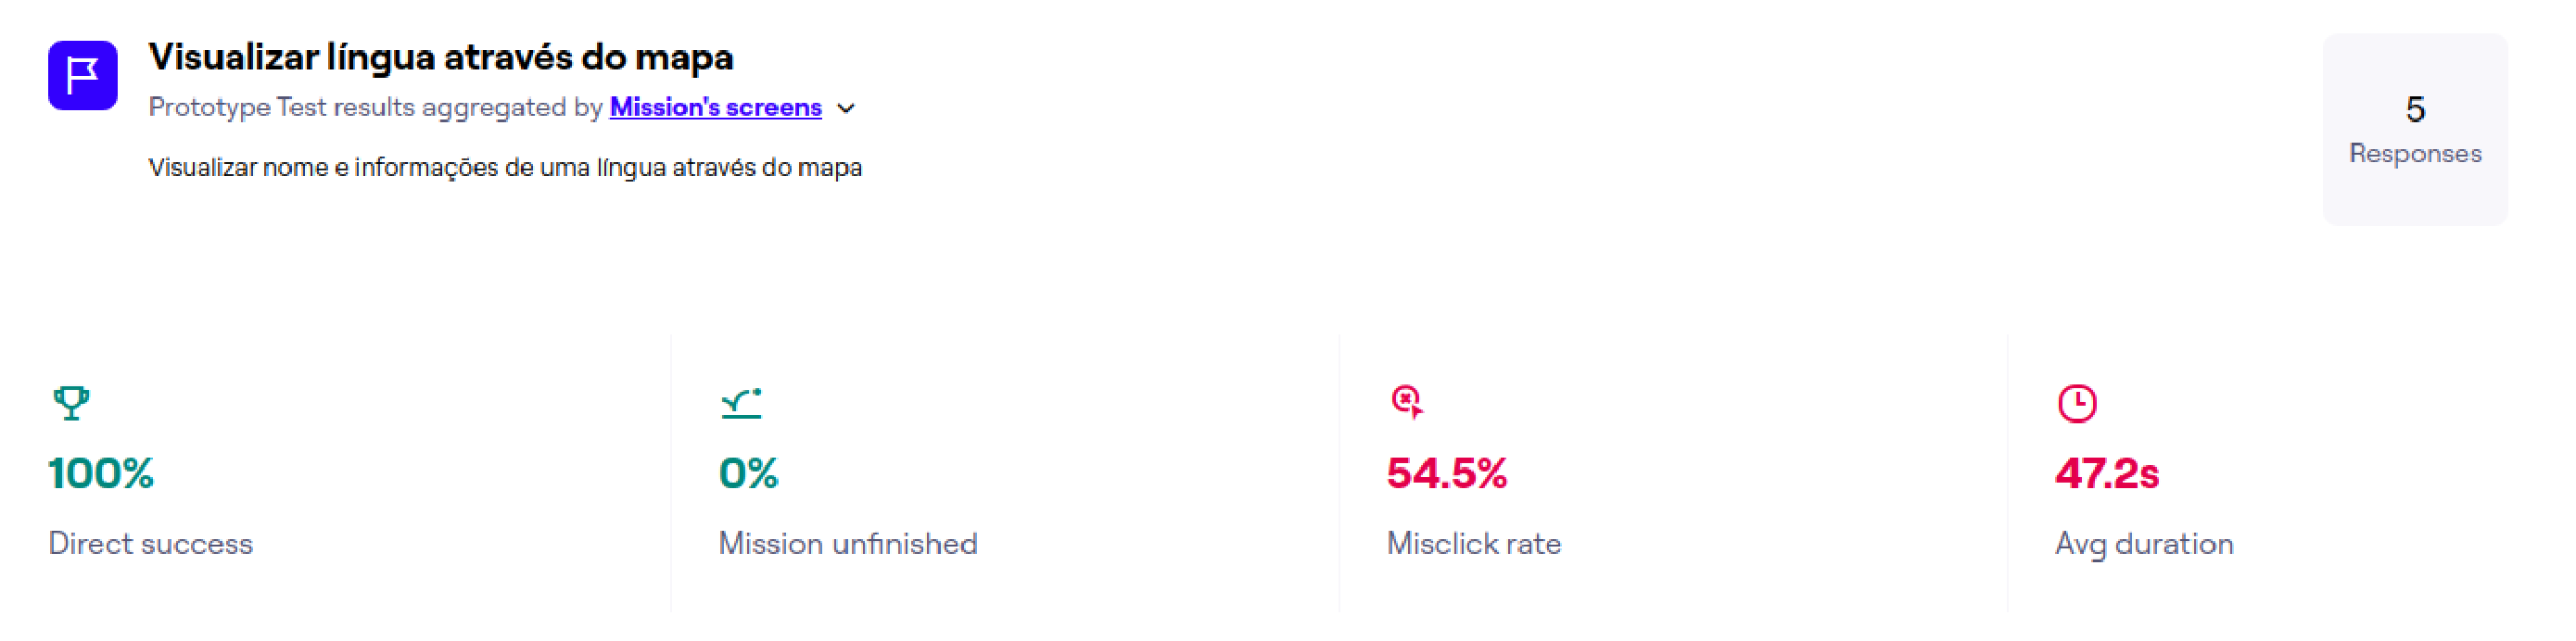
\includegraphics[width=1\textwidth]{figuras/maze.eps}
	\end{adjustbox}
	\begin{tablenotes}[flushleft]
		\centering
		\item \textit{Fonte:} Autora.
	\end{tablenotes}
	\label{fig31}
\end{figure}

A Figura \ref{fig32} fornece informações de sessão específicas por participante, incluindo o tempo gasto durante a execução das tarefas e o resultado obtido, indicando se foi um sucesso direto ou indireto.

O sucesso direto é caracterizado pela capacidade do participante de concluir a tarefa seguindo o caminho esperado, ou seja, o fluxo de telas definido para que o participante complete uma tarefa específica. Por outro lado, o sucesso indireto ocorre quando o usuário completa a tarefa 
sem seguir esse caminho previamente definido, seja passando por um fluxo diferente ou percorrendo um número maior de telas antes de concluir.

\begin{figure}[h!]
	\centering
	\caption{Resultados por participante na plataforma Maze}
	\begin{adjustbox}{center}
		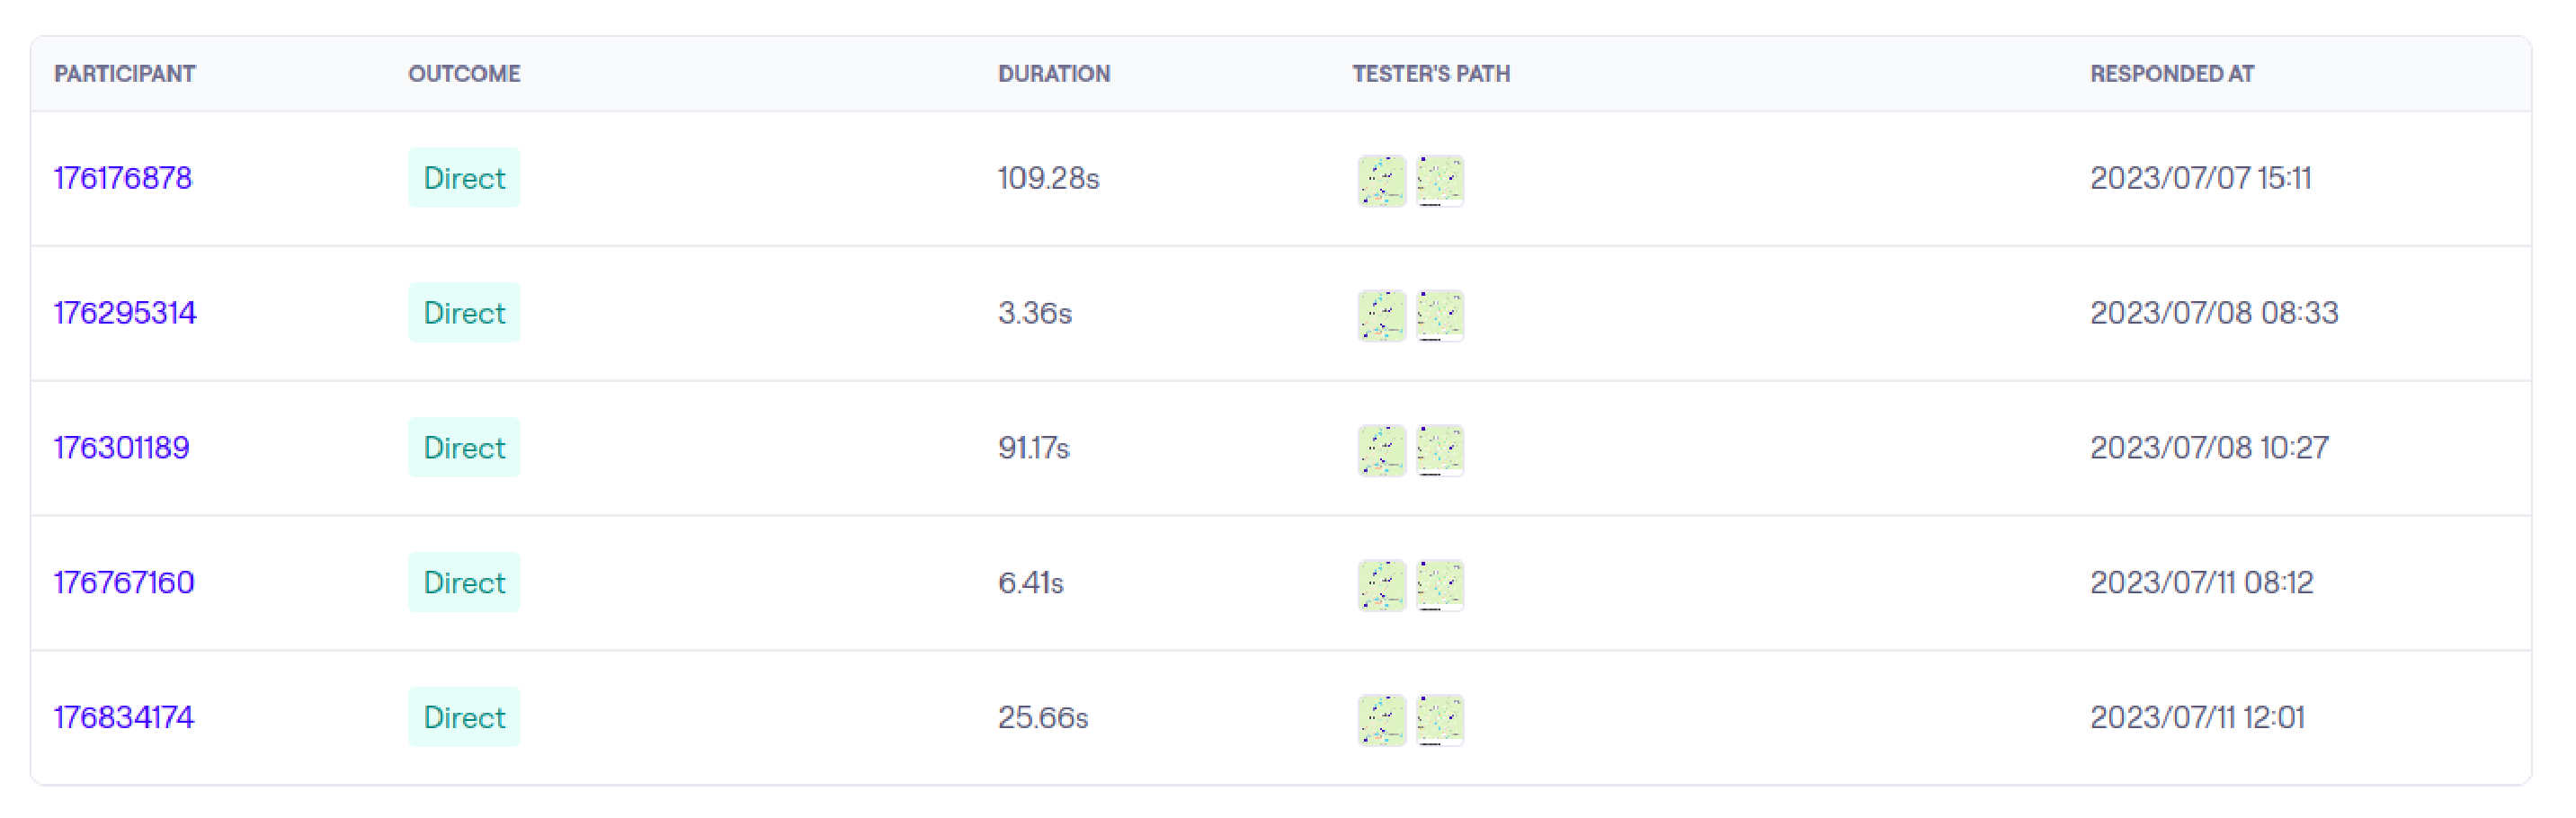
\includegraphics[width=1\textwidth]{figuras/maze2.eps}
	\end{adjustbox}
	\begin{tablenotes}[flushleft]
		\centering
		\item \textit{Fonte:} Autora.
	\end{tablenotes}
	\label{fig32}
\end{figure}

Além disso, ao final dos testes, foi aplicado um questionário baseado no Questionário \textit{Attrakdiff} para avaliar a experiência do usuário no aplicativo Multilind. Este questionário foi detalhadamente explicado na seção \hyperref[sec:Medicao2]{2.3.1}.